% !Mode:: "TeX:UTF-8"

\chapter{实验结果和分析}

\section{实验数据集以及评估标准}

\subsection{实验数据集}

公开数据数据集berkeley segmentation dataset(BSDS500)\cite{arbelaez2010contour}是伯利克里大学computer vision group课题组提供的数据集,已广泛应用于图像分割和物体边缘检测。
该数据集中包含500张图像,其中200张用于训练,100张用于验证以及200张用于测试。
所有的真值用.mat文件保存,包含segmentation和boundaries两种数据信息,每张图片对应真值有五个,为五个人标注的真值。BSDS500已经成为图像分割,超像素分割和边缘检测的标准基准。
本文使用BSDS500数据集中的200张测试图片来进行实验及评估。

\subsection{评估标准}

图像分割和超像素分割是计算机视觉领域重要的两个方向,并且已经有许多公开可用的评估基准。
本小结将介绍本文所使用的图像分割和超像素分割的评估标准。

为了对实验结果进行评估,本文使用Boundary F-measure(BF), Probabilistic Rand Index (PRI)\cite{carpineto2012consensus} 和Global Consistency Error (GCE)\cite{khelifi2016gce}作为图像分割的主要指标。用 BF, Boundary Recall (BR), under segmentation error (UE) 和compactness(CO) 作为超像素分割的主要指标。我们基于整个数据集的整体性能选择最佳参数。 BF,BR,PRI和CO的分值越高,结果越好。 GCE 分值和UE分值越低,结果越好。

对于评估标准BF和BP的计算,本文使用了以下四个数值来进行定义:

\begin{itemize}
\item True Positive,TP:称为真阳性。以边界像素为例,某像素点被预测为边界,在groundtruth中真实分类也为边界;
\item False Positive,FP:称为假阳性,某像素点被预测为边界,但在groundtruth中真实分类不是边界;
\item False Negative,FN:称为假阴性,某像素点被模型不是边界,在groundtruth中真实分类却是边界
\end{itemize}

(1)边界召回率BR可以理解为预测结果中,真正属于边界的像素数目占所有像素数目比例,其计算公式为:
\begin{equation}
BR = \frac{TP}{TP+FN}
\end{equation}

(2)在介绍Boundary F-measure(BF)之前,首先介绍与召回率recall对应的评估指标精确率precision,以边界精确率为例,其含义为预测结果中,真正属于边界的像素数目占预测结果中所有边界像素的比例,计算公式为:
\begin{equation}
BP = \frac{TP}{TP+FP}
\end{equation}

可见,精确率和召回率是相互影响的,理想情况下两者都高,但是一般情况下准确率高,召回率就低;召回率高,准确率就低。
为了平衡这个两个指标,综合衡量P和R,更好的来评估结果,应该使用F值,其计算公式为:
\begin{equation}
F=\frac{(\alpha^{2}+1)\cdot P\cdot R }{\alpha^{2}\cdot(P+R)}
\end{equation}

$\alpha$为1时,就是常见的F1值(F1 score):

\begin{equation}
F1=\frac{2 \cdot P\cdot R }{P+R}
\end{equation}

一般多个模型假设进行比较时,F1 score越高,说明它越好。本文使用的BF就是边界的F1值。

(4)PR曲线 (precision-recall curve):PR曲线的横坐标和纵坐标分别是召回率和准确率。
PR曲线上的的点代表不同阈值下召回率和准确率。
由上述公式可知,准确率和召回率成负相关, 即准确率越高,召回率越小。
对于图像分割的PR曲线,若曲线与X轴和Y轴包含的面积越大,表示分割效果越好,
即得到的曲线形状越靠近右上方,则表示法性越好。

(5)Global Consistency Error (GCE):计算两个区域相互一致的程度,定义为:

假设图像分割结果表示为$S^{t} = \left \{ C_{1}^{t},C_{2}^{t},\cdots ,C_{R^{t}}^{t} \right \}$,groundtruth分割图表示为
$S^{g} = \left \{ C_{1}^{g},C_{2}^{g},\cdots ,C_{R^{g}}^{g} \right \}$。其中,$R^{t}$是$S^{t}$中的区域$C$的数量,$R^{g}$是$S^{g}$中的区域数。

对于特定的像素$p_{i}$,我们考虑$S^{t}$和$S^{g}$中包括该像素的段。 我们分别用$C_{<pi>}^{t}$和$C_{<pi>}^{g}$ 表示这些段。如果一个段是另一段的子集,则像素实际上包含在细化区域中,并且局部误差应等于零。 如果没有子集关系,则这两个区域将以不一致的方式重叠,并且局部误差应不同于零。 因此,局部细化误差(LRE)在像素$p_{i}$处表示为:
\begin{equation}
LER(S^{t},S^{g},p_{i}) = \frac{\left | C_{\left \langle p_{i}\right \rangle}^{t} \setminus
C_{\left \langle p_{i}\right \rangle}^{g}   \right |}{\left | C_{\left \langle p_{i}\right \rangle}^{t}\right |}
\end{equation}

其中$\setminus $表示集合的差运算,而$|C|$代表像素集C的基数。所谓的全局一致性误差(GCE),就是将每个像素处的LRE组合成整个图像的度量,公式如下:
\begin{equation}
GCE(S^{t},S^{g})=\frac{1}{n}\min \left \{ \sum_{i=1}^{n}LRE(S^{t},S^{g},p_i),\sum_{i=1}^{n}LRE(S^{g},S^{t},p_i)     \right \}
\end{equation}
其中n是图像中像素$p_i$的数量。这种基于GCE的分割误差度量,其值属于区间[0,1]。0表示两个分段之间完全匹配,误差为1表示要比较的两个分段之间的最大差值。

(6)PRI是一种相似性度量,它计算分割图像与真实分割之间的一致性。

同样我们假设图像分割结果表示为$S^{t} = \left \{ C_{1}^{t},C_{2}^{t},\cdots ,C_{R^{t}}^{t} \right \}$,
groundtruth 分割图表示为$S^{g} = \left \{ C_{1}^{g},C_{2}^{g},\cdots ,C_{R^{g}}^{g} \right \}$。
其中,$R^{t}$是$S^{t}$中的区域$C$的数量,$R^{g}$是$S^{g}$中的区域数。

the Rand index(RI)定义为:
\begin{equation}
RI = \frac{n_{11}+n_{00}}{n_{00}+n_{01}+n_{10}+n_{11}}
\end{equation}
其中,$n_{11}$表示$S^{t}$和$S^{g}$中位于同一区域中的像素对数。
$n_{00}$表示$S^{t}$和$S^{g}$中位于不同区域中的像素对数。
$n_{10}$表示在$S^{t}$中位于同一区域,而$S^{g}$中位于不同区域中的对象对数。
$n_{01}$表示在$S^{t}$中位于不同区域,而$S^{g}$中位于同一区域的对象对数。

RI方法中,所有参数的权重是相同的,为了更好的平衡各项,PRI对各项进行了加权。

假设每个像素随机分配给一个区域,两个像素在$S^{t}$和$S^{g}$中位于同一个区域的概率为:
\begin{equation}
p_{11}=\frac{1}{R^t} \cdot \frac{1}{R^g}
\end{equation}

两个像素在$S^{t}$和$S^{g}$中的不同区域中的概率是:
\begin{equation}
p_{00}=\frac{R^t-1}{R^t} \cdot \frac{R^g-1}{R^g}
\end{equation}

两个像素在$S^{t}$中位于同一个区域中,而在$S^{g}$中位于不同区域的概率为:
\begin{equation}
p_{10}=\frac{1}{R^t} \cdot \frac{R^g-1}{R^g}
\end{equation}

两个像素在$S^{t}$中位于不同区域,而在$S^{g}$中位于同一个区域的概率为:
\begin{equation}
p_{01}=\frac{R^t-1}{R^t} \cdot \frac{1}{R^g}
\end{equation}

其中$\sum_{h=00}^{11}p_{h}=1$($h$以二进制表示)。概率越低,则事件确实发生的权重就越高。权重计算公式为:
\begin{equation}
w_{h} = -\log_2\left ( p_{h}\right )
\end{equation}

这些权重可用于定义Probabilistic Rand Index:
\begin{equation}
PRI = \frac{w_{11}\cdot n_{11}+w_{00}\cdot n_{00}}
{w_{00}\cdot n_{00}+w_{01}\cdot n_{01}+w_{10}\cdot n_{10}+w_{11}\cdot n_{11}}
\end{equation}

与RI相比,使用PRI的优点在于,对各项进行了权衡。

(7) under segmentation error (UE):欠分割率,UE作为一种超像素分割评估方法,该方法惩罚像素跟真实分割不重合的情况。其本质是衡量算法在根据真实值对图像进行分割时所犯的错误。其计算公式为:

\begin{equation}
UE = \frac{1}{N}\left [ \sum_{i=1}^{R^{g}}(\sum_{\left [ S_{j}|S_{j} \bigcap g_{i}> B \right ]}
\left | S_{j} \right |   )-N   \right ]
\end{equation}
其中,$\left | \cdot \right |$表示此区域内像素的数量,$N$表示图像的大小,(以像素为单位)。B是需要重叠的最小像素数,默认将B设为$\left | S_{j} \right |$的$5\%$,以解决真值分割数据中的小错误。表达式$S_{j} \bigcap g_{i}$是超像素$S_{j}$ 相对于地面真实部分$g_{i}$的相交或重叠误差。

(8)compactness(CO):紧凑度,指标衡量了超像素是否“紧实”。

在数学中,测量形状的紧凑度常用的量度是isoperimetric quotient。
其规定圆形的isoperimetric quotient为1,并且形状变得越不紧凑,值越小。
假设一个超像素的面积为$A_{s}$,周长为$L_{s}$,那么具有与超像素相同的周长的圆的半径为$r = \frac{L_{s}}{2\pi}$。
令$A_C$为半径为$r$的圆的面积,即$A_{c}=\pi r^{2}$。isoperimetric quotient的计算如下:
\begin{equation}
Q_{s} = \frac{A_{s}}{A_{c}} = \frac{4\pi A{s}}{L_{s}^{2}}
\end{equation}
%Measuring and Evaluating the Compactness of Superpixels
基于isoperimetric quotient,Alexander Schick等人提出了一种衡量超像素分割的紧凑度(CO)的度量。 对于给定的图像I,其超像素分割结果为$S = \left \{ S_{1},S_{2},\cdots ,S_{m} \right \}$,分割结果的紧凑度为:
\begin{equation}
CO=\sum_{i=1}^{m}Q_{s_{i}}\cdot \frac{\left | S_{i}\right |}{\left | I\right |}
\end{equation}

\begin{figure*}[h]
\centering
\subfigure[]{
\begin{minipage}[b]{0.3\linewidth}
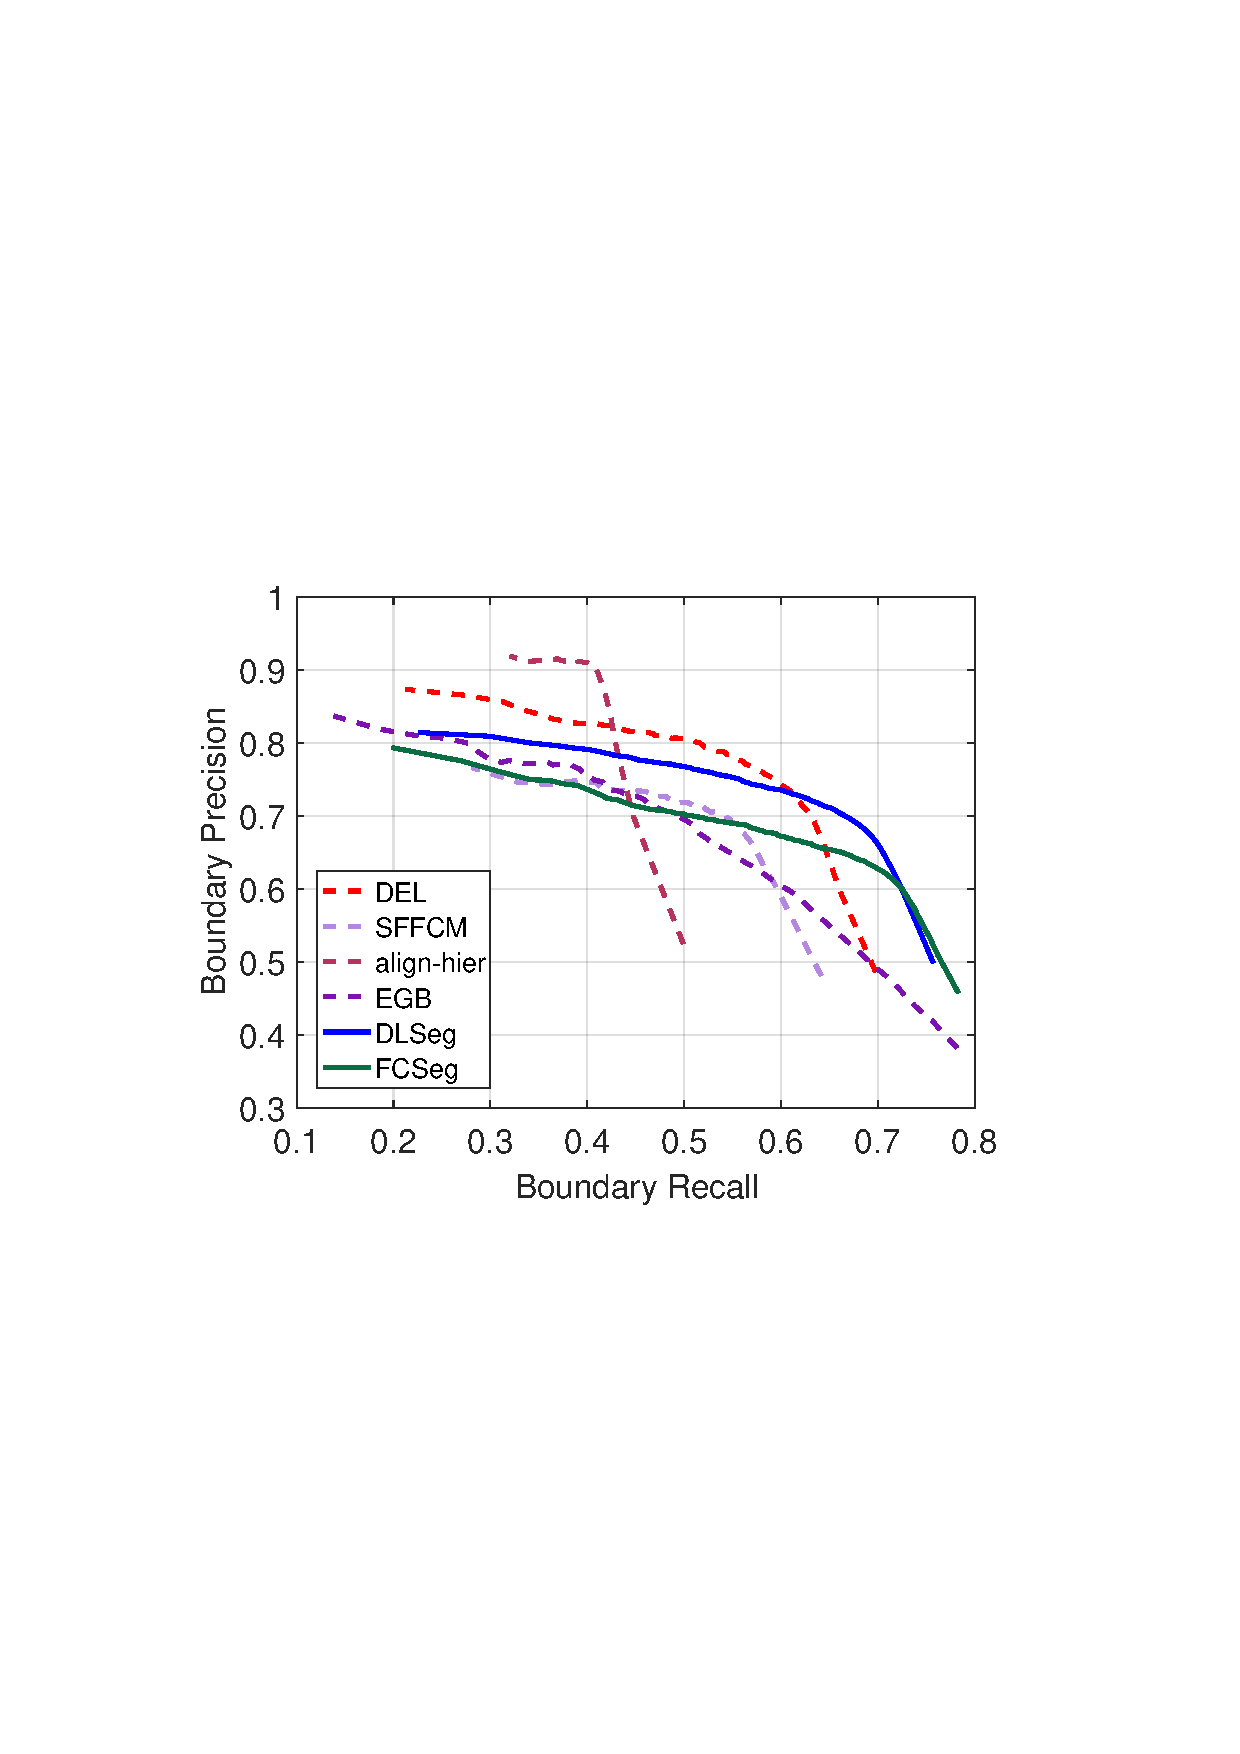
\includegraphics[width=1\linewidth]{figures/img/Chart/fig1_1.pdf}
\end{minipage}}
\hspace{-2.5mm}
\subfigure[]{
\begin{minipage}[b]{0.3\linewidth}
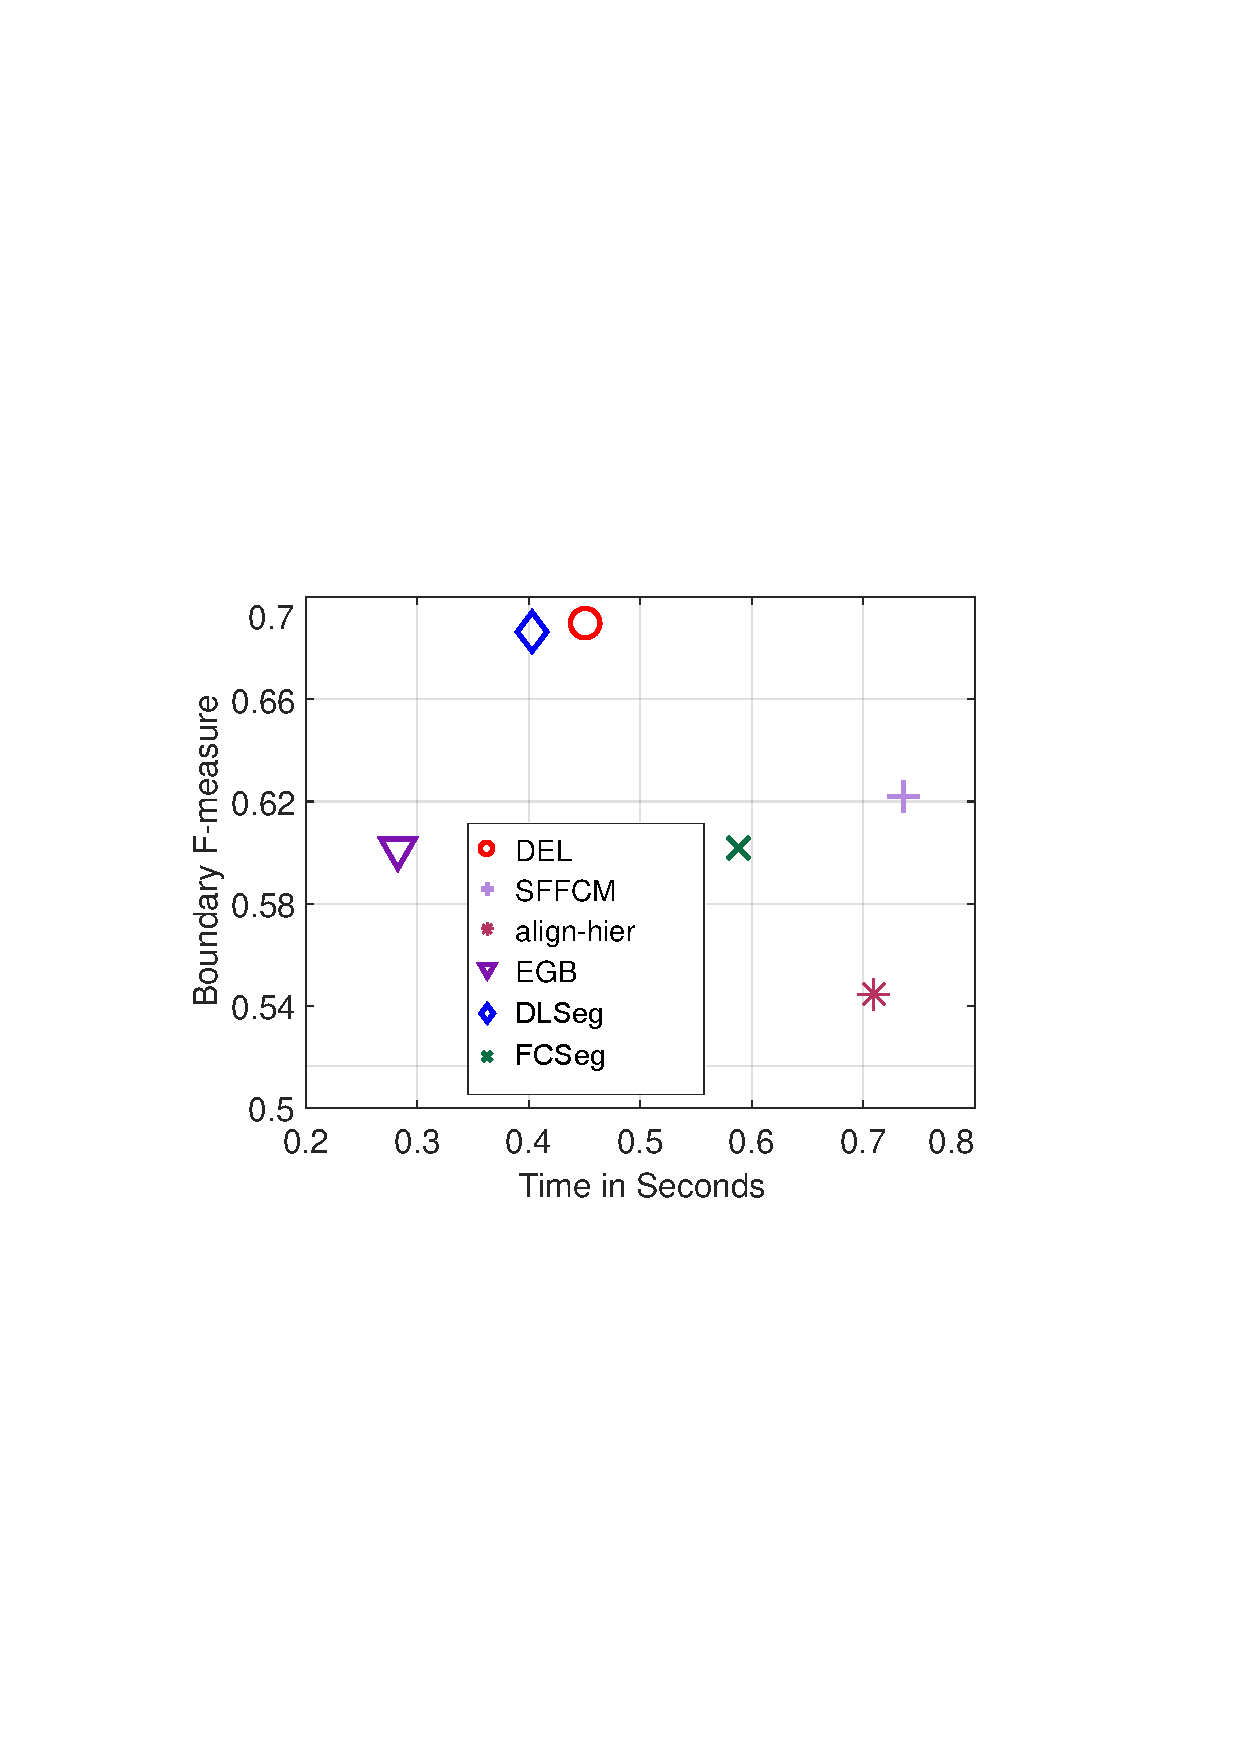
\includegraphics[width=1\linewidth]{figures/img/Chart/fig1_2.pdf}
\end{minipage}}
\hspace{-2.5mm}
\subfigure[]{
\begin{minipage}[b]{0.3\linewidth}
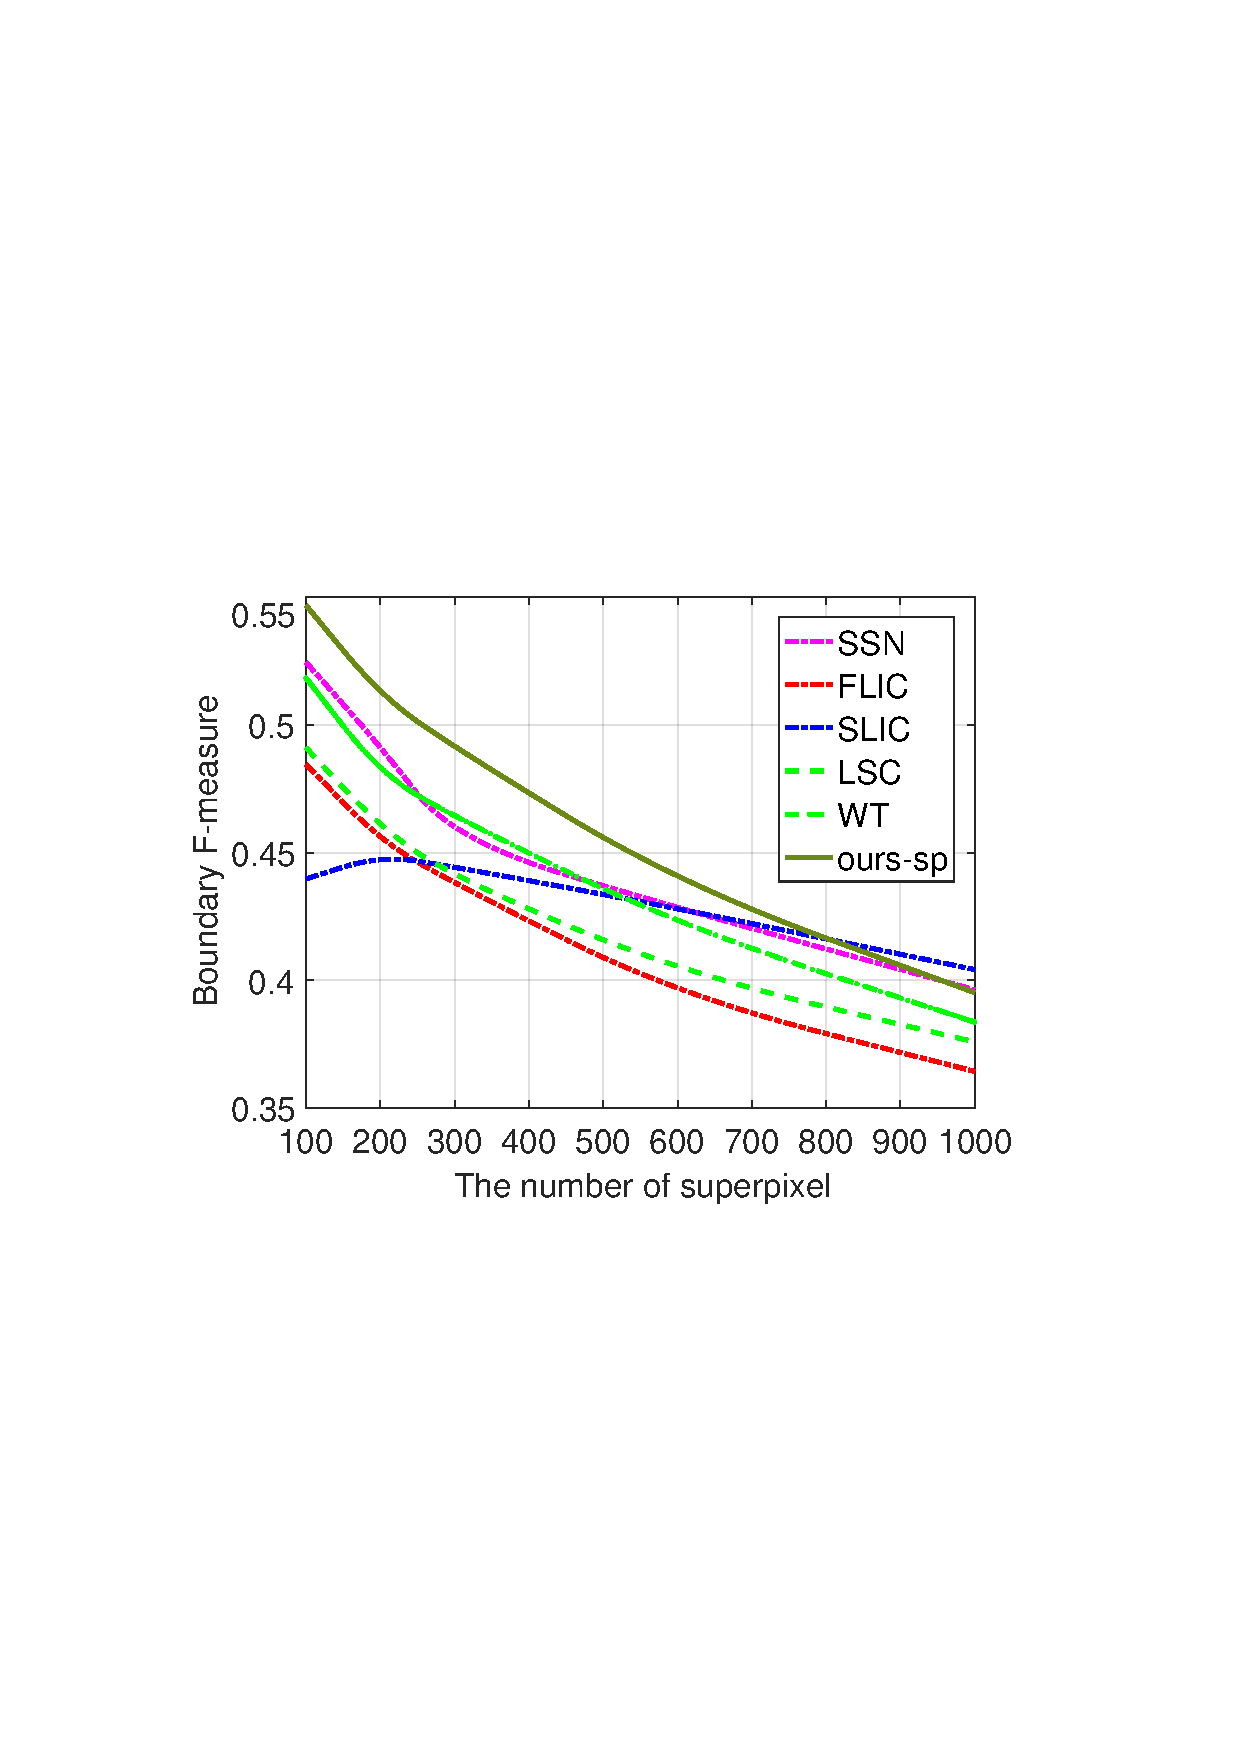
\includegraphics[width=1\linewidth]{figures/img/Chart/fig1_3.pdf}
\end{minipage}}
%\vspace{-7mm}
\caption{BSDS500数据集上的结果对比。\textbf{左}:图像分割算法的边界P-R曲线图,\textbf{中}:图像分割算法的BF和时间比较,\textbf{右}:超像素分割算法的BF值比较}
\label{Fig5.1}
\end{figure*}

\section{消融实验}

\subsection{基于深度学习的超像素分割和图像分割}
\subsubsection{实验介绍}

我们使用图\ref{fig3.1}中的网络结构作为我们的基本结构,将其命名为DLSeg-GN8。我们用BSDS500 数据集来测试网络中每个组件的不同选择。除了ours-GN8模型,从超像素分割和图像分割两方面,我们将ours-GN8分别和其他4种变形进行了比较。

1. DLSeg-BN: 用batch normalization(BN)操作代替group normalization(GN)操作。

2. DLSeg-GN32: 在GN操作中,将group number参数设为32,而不是ours-GN8模型中的参数8。

3. DLSeg-conv7:对于超像素分割和图像分割,我们使用同一个特征,即从conv7中获取到的特征。

4.DLSeg-w/o-concat:舍弃conv2$\rightarrow$ concat和conv4$\rightarrow$concat两个过程,即不包含从conv2和conv4 获取到的特征。

在下面一节中,我们将评估图像分割和超像素分割的结果。

\subsubsection{实验结果以及数据分析}

\begin{table}[htbp]
\caption{The performance of superpixel generation of 4 variants}
\label{tab1}
\vspace{0.5em}\centering\wuhao
\begin{tabular}{ccccc}
\toprule[1.5pt]
Methods & BF($\uparrow$) & BR($\uparrow$) & UE($\downarrow$) & CO($\uparrow$) \\
\midrule[1pt]
DLSeg-BN         & 0.547 & 0.884 & 0.068 & 0.373\\
DLSeg-GN32       & 0.546 & 0.897 & 0.066 & 0.376\\
DLSeg-conv7      & 0.521 & 0.812 & 0.094 & 0.413\\
DLSeg-w/o-concat & 0.521 & 0.895 & 0.071 & 0.340\\
\midrule[1pt]
DLSeg-GN8        & 0.547 & 0.918 & 0.065 & 0.316\\
\bottomrule[1.5pt]
\end{tabular}
\end{table}

\begin{table}[htbp]
\caption{The performance of image segmentation of 4 variants}
\label{tab2}
\vspace{0.5em}\centering\wuhao
\begin{tabular}{cccc}
\toprule[1.5pt]
Methods & BF($\uparrow$) & PRI($\uparrow$) & GCE($\downarrow$) \\
\midrule[1pt]
DLSeg-BN          & 0.661 & 0.807 & 0.146 \\
DLSeg-GN32        & 0.685 & 0.820 & 0.171 \\
DLSeg-conv7       & 0.492 & 0.714 & 0.088\\
DLSeg-w/o-concat  & 0.560 & 0.817 & 0.182 \\
\midrule[1pt]
DLSeg-GN8         & 0.686 & 0.822 & 0.170 \\
\bottomrule[1.5pt]
\end{tabular}
\vspace{\baselineskip}
\end{table}

表\ref{tab1}展示了五种模型在超像素分割方面的对比结果,表\ref{tab2}展示了五种模型在图像分割方面的对比结果。
从表\ref{tab1}和表\ref{tab2}可知,相对于其他4种变体而言,DLSeg-GN8模型性能表现最好,验证了我们选择组件的合理性。

DLSeg-GN8模型和DLSeg-GN32模型相对于DLSeg-BN模型而言,在超像素分割和图像分割的边界保持方面更有优势。
GN操作解决了BN操作对批次大小依赖性的影响。对于小批次,GN操作可以取得更好的效果。
但是DLSeg-GN32模型的效果较DLSeg-GN8模型的效果有所降低。
当分组数量过大的时候,效果有所下降。

在卷积神经网络中,浅层网络包含更详细的信息,而深层网络包含更多的全局信息。
因为DLSeg-GN8模型比DLSeg-w/o-concat模型包含更多提取到的特征,因此分割效果更好。
DLSeg-conv7 的分割效果明显降低,DLSeg-GN8远远好于DLSeg-conv7,从而证明在多任务学习中,不同级别的任务需要不同的图像特征。

\subsection{基于Boruvka算法和快速模糊C均值聚类的图像分割}

为了确定不同超像素数目对最终图像分割结果的影响,本文将基于Boruvka算法产生的超像素数目N分别设置为8,10,20,50,100,300,来进行实验。此外为了验证快速模糊C均值聚类方法的有效性,设置了对照组--FCSeg-Boruvka,该模型只使用Boruvka进行分割来进行分割图像,不使用快速模糊C 均值聚类。实验数据如表\ref{tab3} 所示。为了方便表示本文将该方法表示为FCSeg。

\begin{table}[htbp]
\caption{The performance of image segmentation of 4 variants}
\label{tab3}
\vspace{0.5em}\centering\wuhao
\begin{tabular}{cccc}
\toprule[1.5pt]
Methods & BF($\uparrow$) & PRI($\uparrow$) & GCE($\downarrow$) \\
\midrule[1pt]
FCSeg-Boruvka   & 0.460 & 0.696 & 0.339 \\
FCSeg-8   & 0.531 & 0.711 & 0.372  \\
FCSeg-10   & 0.537 & 0.717 & 0.352 \\
FCSeg-20   & 0.571 & 0.724 & 0.306 \\
FCSeg-50  & 0.580 & 0.735 &  0.268 \\
FCSeg-100  & 0.594 & 0.736 &  0.241\\
FCSeg-300  & 0.576 & 0.720 &  0.280\\
\bottomrule[1.5pt]
\end{tabular}
\vspace{\baselineskip}
\end{table}

从表中可以看出,FCSeg-Boruvka模型效果不佳,证明了基于Boruvka算法和快速模糊C均值聚类方法的合理性以及有效性。
当超像素小于100时,分割效果随着超像素数量的增加而变好,
但是当超像素数量超过100个时,分割效果就会越来越差。
由经验可知,但超像素数量过高,每个超像素内包含的像素数量极少,超像素对边界的保持性降低,
分割效果将会降低。
故而,选择$N_{sp}=100$作为超像素的数量。

\begin{figure*}[h]
\centering
\subfigure[GT]{
\begin{minipage}[b]{0.13\linewidth}
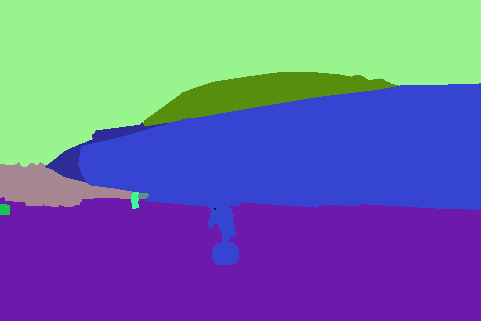
\includegraphics[width=1\linewidth]{figures/img/gt/gt_10081.png}

\includegraphics[width=1\linewidth]{figures/img/gt/gt_43051.png}

\includegraphics[width=1\linewidth]{figures/img/gt/gt_80085.png}

\includegraphics[width=1\linewidth]{figures/img/gt/gt_92014.png}
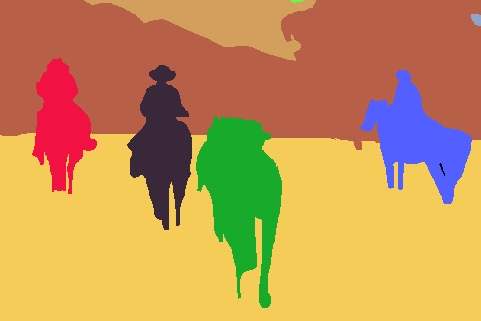
\includegraphics[width=1\linewidth]{figures/img/gt/gt_220003.png}
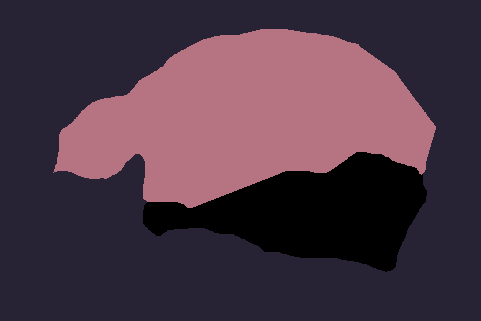
\includegraphics[width=1\linewidth]{figures/img/gt/gt_176051.png}
\end{minipage}}
\hspace{-2.2mm}
\subfigure[SSN]{
\begin{minipage}[b]{0.13\linewidth}
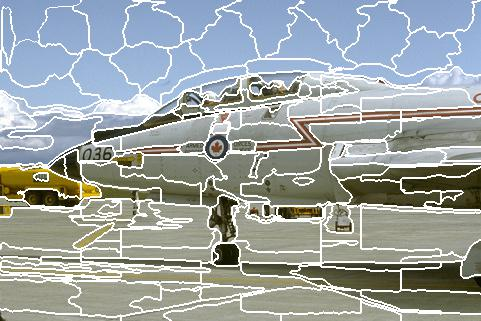
\includegraphics[width=1\linewidth]{figures/img/SSN/SSN_10081.jpg}
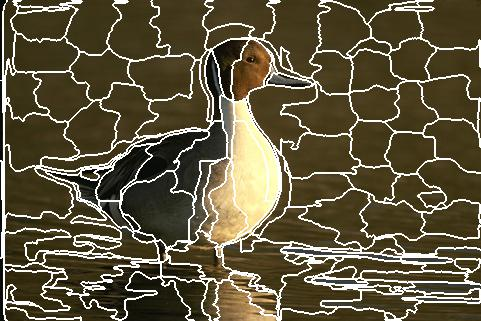
\includegraphics[width=1\linewidth]{figures/img/SSN/SSN_43051.jpg}
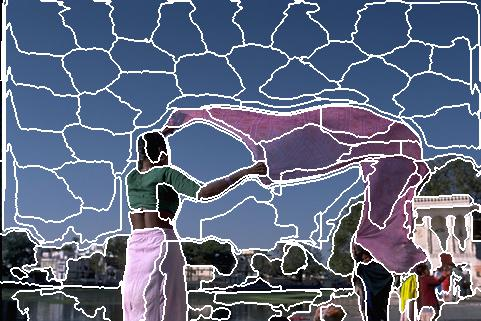
\includegraphics[width=1\linewidth]{figures/img/SSN/SSN_80085.jpg}
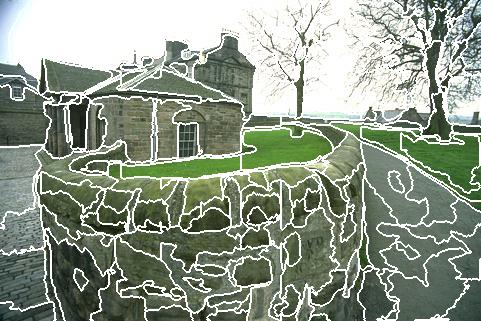
\includegraphics[width=1\linewidth]{figures/img/SSN/SSN_92014.jpg}
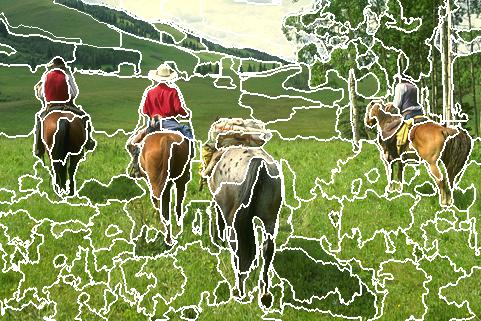
\includegraphics[width=1\linewidth]{figures/img/SSN/SSN_220003.jpg}
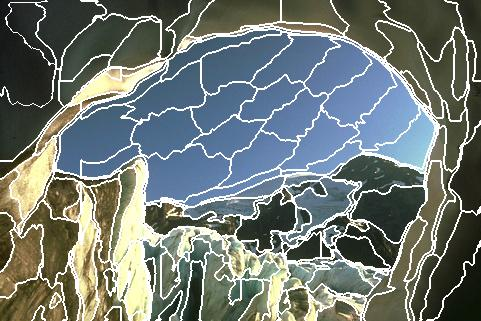
\includegraphics[width=1\linewidth]{figures/img/SSN/SSN_176051.jpg}
\end{minipage}}
\hspace{-2.2mm}
\subfigure[FLIC]{
\begin{minipage}[b]{0.13\linewidth}
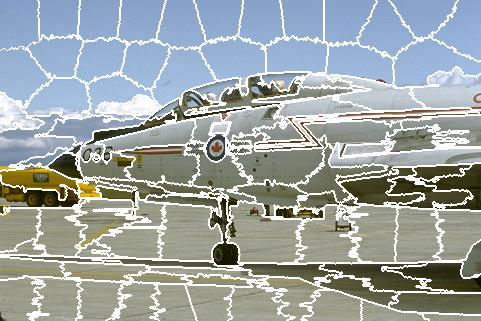
\includegraphics[width=1\linewidth]{figures/img/FLIC/FLIC_10081.jpg}
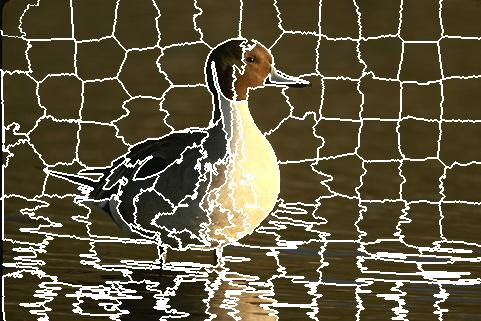
\includegraphics[width=1\linewidth]{figures/img/FLIC/FLIC_43051.jpg}
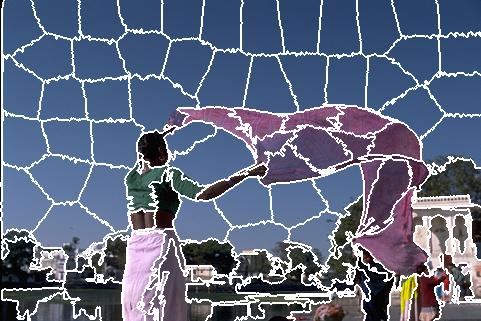
\includegraphics[width=1\linewidth]{figures/img/FLIC/FLIC_80085.jpg}
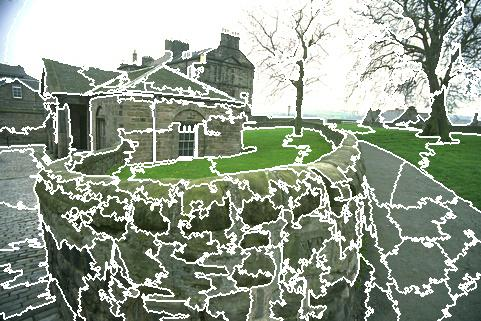
\includegraphics[width=1\linewidth]{figures/img/FLIC/FLIC_92014.jpg}
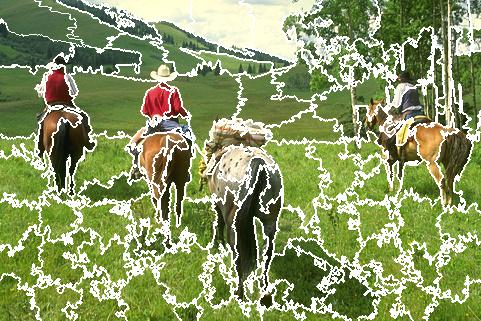
\includegraphics[width=1\linewidth]{figures/img/FLIC/FLIC_220003.jpg}
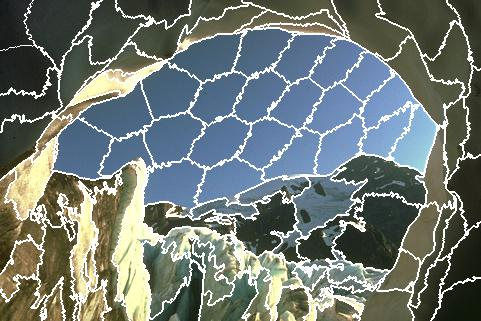
\includegraphics[width=1\linewidth]{figures/img/FLIC/FLIC_176051.jpg}
\end{minipage}}
\hspace{-2.2mm}
% SLIC
\subfigure[SLIC]{
\begin{minipage}[b]{0.13\linewidth}
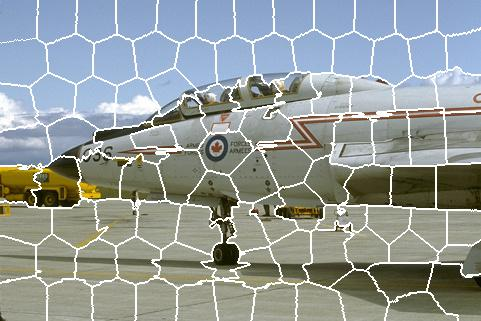
\includegraphics[width=1\linewidth]{figures/img/SLIC/SLIC_10081.jpg}
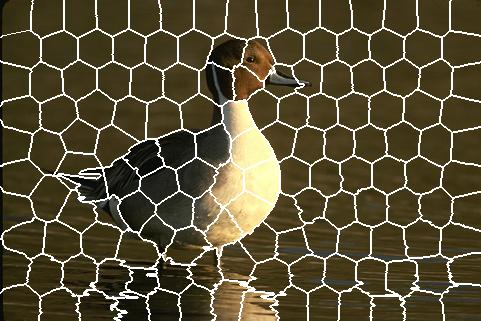
\includegraphics[width=1\linewidth]{figures/img/SLIC/SLIC_43051.jpg}
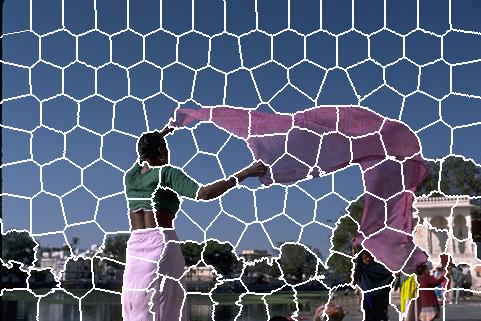
\includegraphics[width=1\linewidth]{figures/img/SLIC/SLIC_80085.jpg}
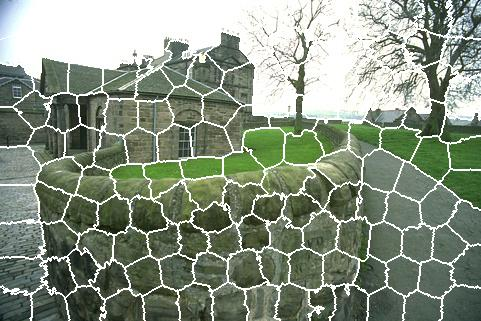
\includegraphics[width=1\linewidth]{figures/img/SLIC/SLIC_92014.jpg}
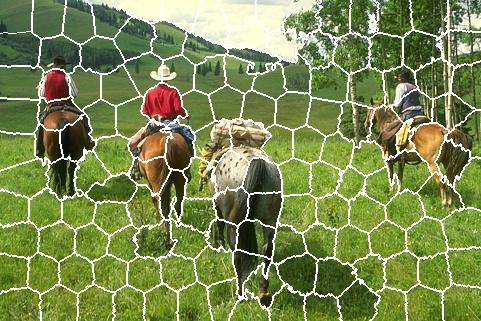
\includegraphics[width=1\linewidth]{figures/img/SLIC/SLIC_220003.jpg}
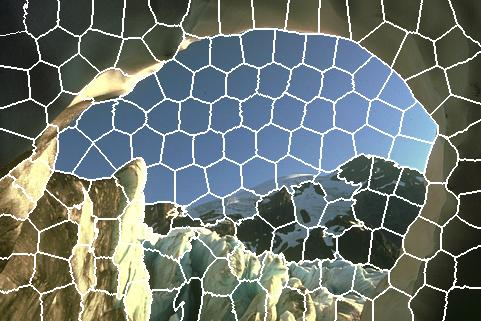
\includegraphics[width=1\linewidth]{figures/img/SLIC/SLIC_176051.jpg}
\end{minipage}}
\hspace{-2.2mm}
\subfigure[LSC]{
\begin{minipage}[b]{0.13\linewidth}
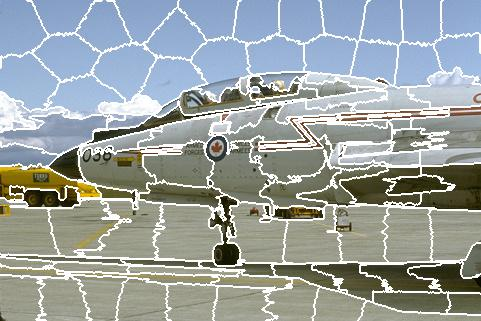
\includegraphics[width=1\linewidth]{figures/img/LSC/LSC_10081.jpg}
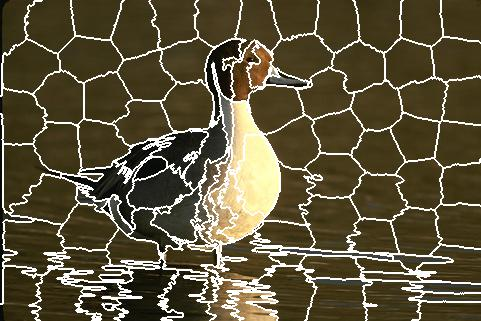
\includegraphics[width=1\linewidth]{figures/img/LSC/LSC_43051.jpg}
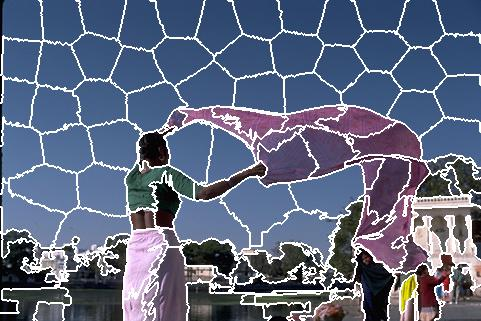
\includegraphics[width=1\linewidth]{figures/img/LSC/LSC_80085.jpg}
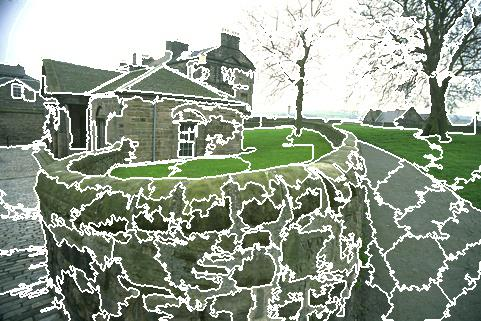
\includegraphics[width=1\linewidth]{figures/img/LSC/LSC_92014.jpg}
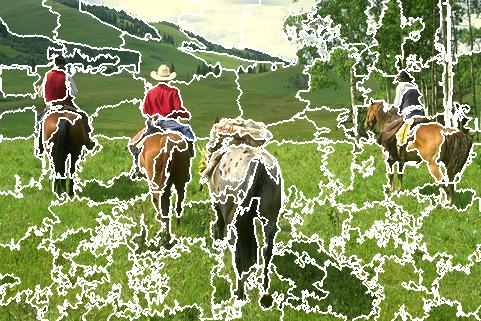
\includegraphics[width=1\linewidth]{figures/img/LSC/LSC_220003.jpg}
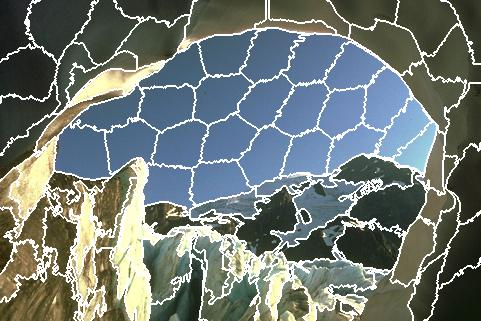
\includegraphics[width=1\linewidth]{figures/img/LSC/LSC_176051.jpg}
\end{minipage}}
\hspace{-2.2mm}
%WT
\subfigure[WT]{
\begin{minipage}[b]{0.13\linewidth}
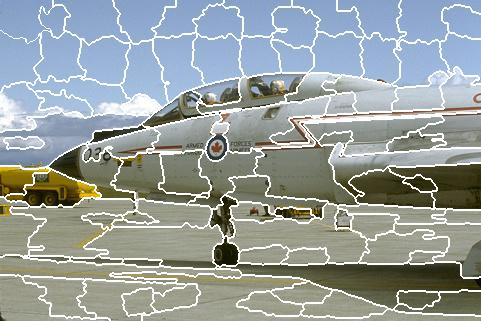
\includegraphics[width=1\linewidth]{figures/img/WT/WT_10081.jpg}
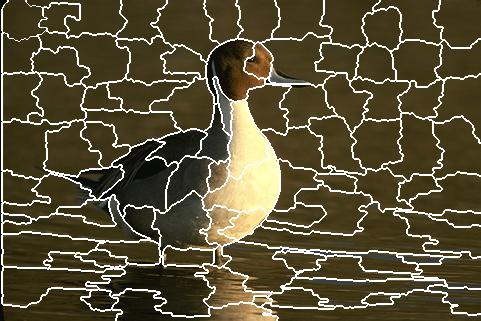
\includegraphics[width=1\linewidth]{figures/img/WT/WT_43051.jpg}
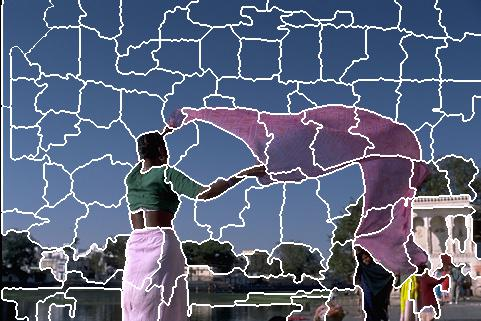
\includegraphics[width=1\linewidth]{figures/img/WT/WT_80085.jpg}
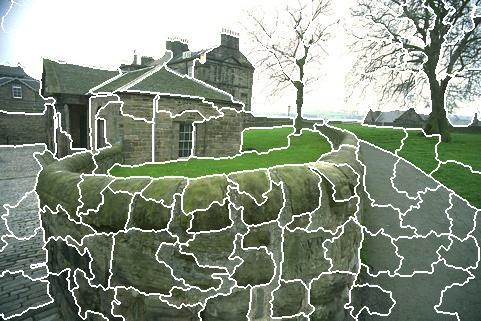
\includegraphics[width=1\linewidth]{figures/img/WT/WT_92014.jpg}
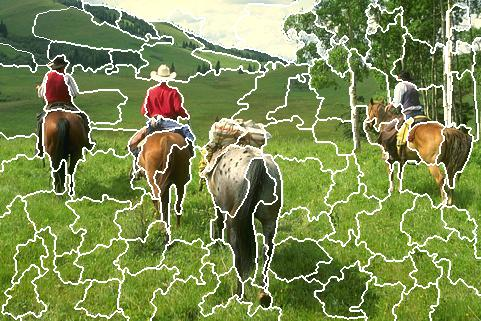
\includegraphics[width=1\linewidth]{figures/img/WT/WT_220003.jpg}
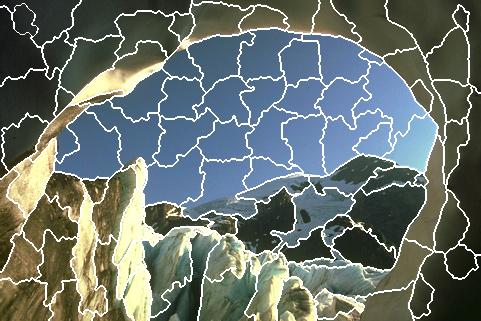
\includegraphics[width=1\linewidth]{figures/img/WT/WT_176051.jpg}
\end{minipage}}
\hspace{-2.2mm}
% ours
\subfigure[DLSeg-sp]{
\begin{minipage}[b]{0.13\linewidth}
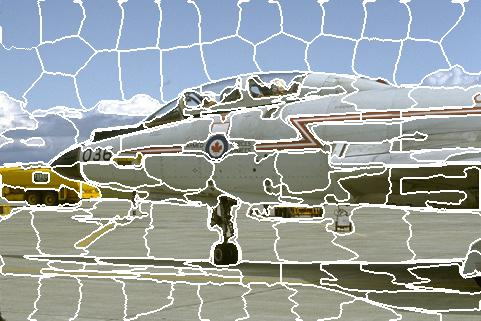
\includegraphics[width=1\linewidth]{figures/img/ours_sp/ourssp_10081.jpg}
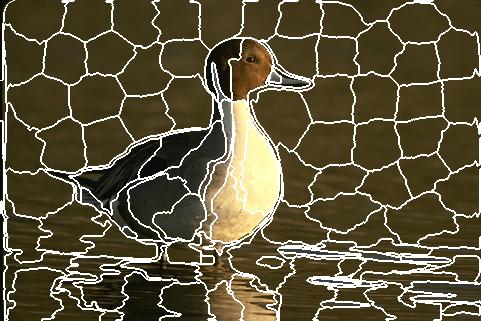
\includegraphics[width=1\linewidth]{figures/img/ours_sp/ourssp_43051.jpg}
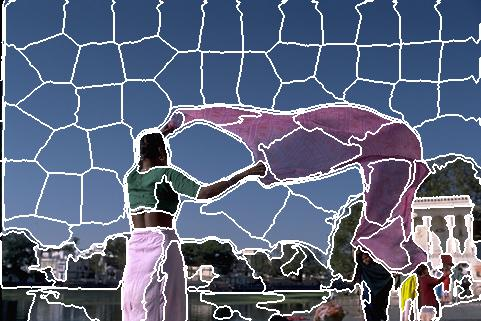
\includegraphics[width=1\linewidth]{figures/img/ours_sp/ourssp_80085.jpg}
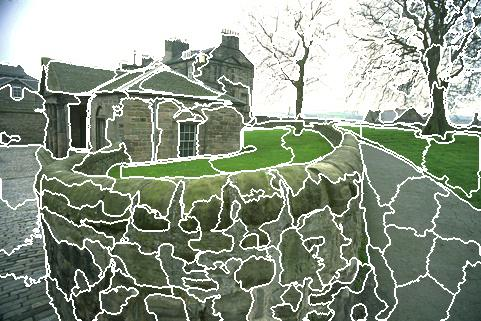
\includegraphics[width=1\linewidth]{figures/img/ours_sp/ourssp_92014.jpg}
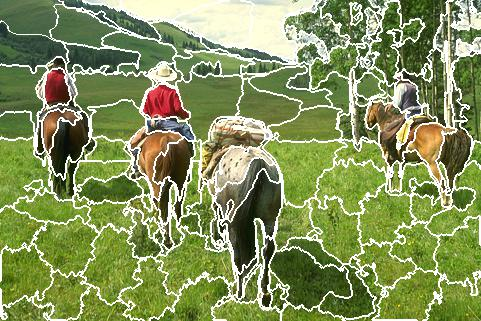
\includegraphics[width=1\linewidth]{figures/img/ours_sp/ourssp_220003.jpg}
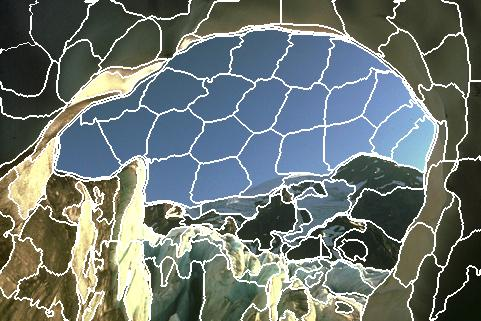
\includegraphics[width=1\linewidth]{figures/img/ours_sp/ourssp_176051.jpg}
\end{minipage}}
%\hspace{-2.2mm}
\caption{超像素分割。第一列显示来自BSDS500数据集的groundtruth。最后六列分别展示了由SSN、FLIC、SLIC、LSC、WT 和我们的方法生成的结果。}
\label{fig5.2}
\end{figure*}

\begin{figure*}[h]
\centering
% input
\subfigure[input]{
\begin{minipage}[b]{0.13\linewidth}
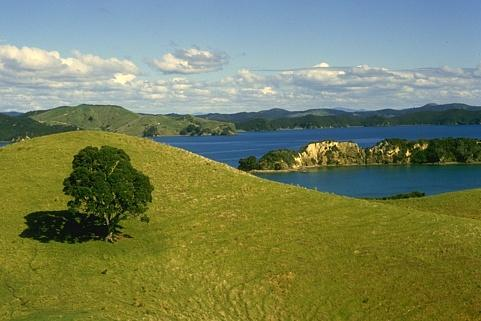
\includegraphics[width=1\linewidth]{figures/img/image/36046.jpg}
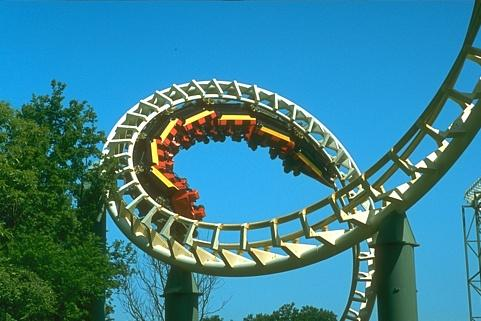
\includegraphics[width=1\linewidth]{figures/img/image/235098.jpg}
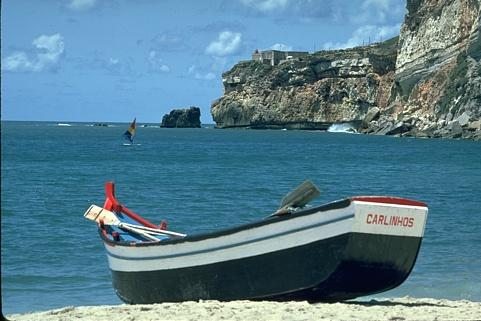
\includegraphics[width=1\linewidth]{figures/img/image/384022.jpg}
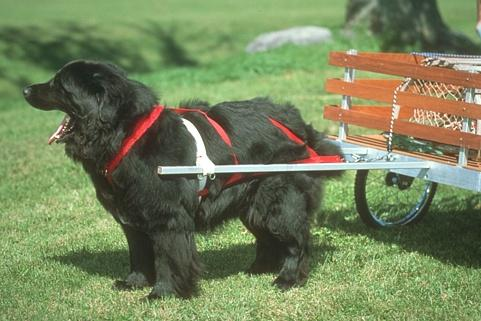
\includegraphics[width=1\linewidth]{figures/img/image/247012.jpg}
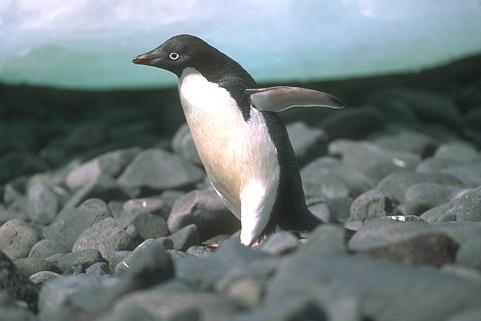
\includegraphics[width=1\linewidth]{figures/img/image/106005.jpg}
\includegraphics[width=1\linewidth]{figures/img/image/5096.jpg}
\end{minipage}}
\hspace{-2.2mm}
% DEL
\subfigure[DEL]{
\begin{minipage}[b]{0.13\linewidth}
\includegraphics[width=1\linewidth]{figures/img/DEL/DEL_36046.png}
\includegraphics[width=1\linewidth]{figures/img/DEL/DEL_235098.png}
\includegraphics[width=1\linewidth]{figures/img/DEL/DEL_384022.png}
\includegraphics[width=1\linewidth]{figures/img/DEL/DEL_247012.png}
\includegraphics[width=1\linewidth]{figures/img/DEL/DEL_106005.jpg}
\includegraphics[width=1\linewidth]{figures/img/DEL/DEL_5096.png}
\end{minipage}}
\hspace{-2.2mm}
% SFFCM
\subfigure[SFFCM]{
\begin{minipage}[b]{0.13\linewidth}
\includegraphics[width=1\linewidth]{figures/img/SFFCM/SFFCM_36046.jpg}
\includegraphics[width=1\linewidth]{figures/img/SFFCM/SFFCM_235098.jpg}
\includegraphics[width=1\linewidth]{figures/img/SFFCM/SFFCM_384022.jpg}
\includegraphics[width=1\linewidth]{figures/img/SFFCM/SFFCM_247012.jpg}
\includegraphics[width=1\linewidth]{figures/img/SFFCM/SFFCM_106005.jpg}
\includegraphics[width=1\linewidth]{figures/img/SFFCM/SFFCM_5096.jpg}
\end{minipage}}
\hspace{-2.2mm}
% SFFCM
\subfigure[align-hier]{
\begin{minipage}[b]{0.13\linewidth}
\includegraphics[width=1\linewidth]{figures/img/align/align_36046.jpg}
\includegraphics[width=1\linewidth]{figures/img/align/align_235098.jpg}
\includegraphics[width=1\linewidth]{figures/img/align/align_384022.jpg}
\includegraphics[width=1\linewidth]{figures/img/align/align_247012.jpg}
\includegraphics[width=1\linewidth]{figures/img/align/align_106005.jpg}
\includegraphics[width=1\linewidth]{figures/img/align/align_5096.jpg}
\end{minipage}}
\hspace{-2.2mm}
% EGB
\subfigure[EGB]{
\begin{minipage}[b]{0.13\linewidth}
\includegraphics[width=1\linewidth]{figures/img/EGB/EGB_36046.jpg}
\includegraphics[width=1\linewidth]{figures/img/EGB/EGB_235098.jpg}
\includegraphics[width=1\linewidth]{figures/img/EGB/EGB_384022.jpg}
\includegraphics[width=1\linewidth]{figures/img/EGB/EGB_247012.jpg}
\includegraphics[width=1\linewidth]{figures/img/EGB/EGB_106005.jpg}
\includegraphics[width=1\linewidth]{figures/img/EGB/EGB_5096.jpg}
\end{minipage}}
\hspace{-2.2mm}
% ours
\subfigure[DLSeg]{
\begin{minipage}[b]{0.13\linewidth}
\includegraphics[width=1\linewidth]{figures/img/ours_seg/ours_36046.jpg}
\includegraphics[width=1\linewidth]{figures/img/ours_seg/ours_235098.jpg}
\includegraphics[width=1\linewidth]{figures/img/ours_seg/ours_384022.jpg}
\includegraphics[width=1\linewidth]{figures/img/ours_seg/ours_247012.jpg}
\includegraphics[width=1\linewidth]{figures/img/ours_seg/ours_106005.jpg}
\includegraphics[width=1\linewidth]{figures/img/ours_seg/ours_5096.jpg}
\end{minipage}}
\hspace{-2.2mm}
\subfigure[FCSeg]{
\begin{minipage}[b]{0.13\linewidth}
\includegraphics[width=1\linewidth]{figures/img/make2/make2_36046.jpg}
\includegraphics[width=1\linewidth]{figures/img/make2/make2_235098.jpg}
\includegraphics[width=1\linewidth]{figures/img/make2/make2_384022.jpg}
\includegraphics[width=1\linewidth]{figures/img/make2/make2_247012.jpg}
\includegraphics[width=1\linewidth]{figures/img/make2/make2_106005.jpg}
\includegraphics[width=1\linewidth]{figures/img/make2/make2_5096.jpg}
\end{minipage}}
\hspace{-2.2mm}
\caption{图像分割。第一列显示来自BSDS500数据集的原始图像和背景真相。最后五列分别显示了DEL、SFFCM、align-hier、EGB 和我们的方法生成的结果。}
\label{fig5.3}
\end{figure*}

\section{对比实验}

\subsection{对比算法}

为了评估我们算法的有效性,我们将从超像素和图像分割两方面与一些最先进的分割算法进行比较,例如SSN\cite{jampani2018superpixel},FLIC\cite{Zhao2017FLIC},SLIC \cite{achanta2012slic},LSC\cite{li2015superpixel},WT\cite{Hu2015Watershed},DEL\cite{liu2018deep},
SFFCM\cite{lei2018superpixel},align-hier\cite{chen2016scale},EGB\cite{felzenszwalb2004efficient}。 其中,SSN,FLIC,SLIC,LSC和WT 是超像素算法。 DEL,SFFCM,align-hier和EGB是图像分割算法。

\subsection{实验结果以及数据分析}

\begin{table}[htbp]
\caption{对比实验:超像素分割性能对比}
\label{tab4}
\vspace{0.5em}\centering\wuhao
\begin{tabular}{ccccc}
\toprule[1.5pt]
Methods & BF($\uparrow$) & BR($\uparrow$) & UE($\downarrow$) & compactness($\uparrow$) \\
\midrule[1pt]
SSN     & \underline{0.524} & \underline{0.911} & \textbf{0.060}    & 0.340 \\
FLIC    & 0.485             & 0.845             & 0.141             & 0.249\\
SLIC    & 0.440             & 0.552             & 0.145             & \textbf{0.661}\\
LSC     & 0.491             & 0.873             & 0.095             & 0.288\\
WT      & 0.518             & 0.837             & 0.124             & \underline{0.438} \\
DLSeg-sp & \textbf{0.547}    & \textbf{0.918}    & \underline{0.065} & 0.316\\
\bottomrule[1.5pt]
\end{tabular}
%\vspace{\baselineskip}
\end{table}

\begin{table}[htbp]
\caption{The performance of image segmentation of 4 variants}
\label{tab5}
\vspace{0.5em}\centering\wuhao
\begin{tabular}{cccc}
\toprule[1.5pt]
Methods & BF($\uparrow$) & PRI($\uparrow$) & GCE($\downarrow$) \\
\midrule[1pt]
DEL        & \textbf{0.689}    & \underline{0.809}  & \underline{0.161}\\
SFFCM      & 0.622             & 0.776              & 0.259\\
align-hier & 0.545             & 0.738              & \textbf{0.141} \\
EGB        & 0.602             & 0.763              & 0.244\\
DLSeg   & \underline{0.686} & \textbf{0.821}     & 0.170 \\
FCSeg  & 0.594 & 0.720 & 0.241 \\
\bottomrule[1.5pt]
\end{tabular}
\vspace{\baselineskip}
\end{table}

对于超像素分割和图像分割,我们将这两个任务与经典算法在BSDS500数据集进行了比较。
图\ref{Fig5.1}显示了我们的算法与其他算法的比较。
左图和中间图显示了我们算法的变体与其他图像分割算法之间的结果比较。
可以看出,DLSeg算法在图像分割中表现良好,并且在BF值和时间方面优于其他算法。
尽管EGB算法花费的时间最少,却效果不佳。
DEL算法在BF值上达到最佳,但在时间方面,较我们的算法有所欠缺。
图\ref{Fig5.1}的最后一个子图显示了DLSeg方法中产生的超像素和其他超像素算法之间的比较。
可以看出,DLSeg方法获得的超像素在BF值上实现了最佳性能。
总而言之,在超像素分割和图像分割两方面,DLSeg算法实现了时间与效果之间的平衡。

表\ref{tab4}和表\ref{tab5}更详细的说明在超像素分割和图像分割两方面的定量比较(前两名分别以粗体和下划线突出显示)。
与其他超像素分割算法相比,尽管DLSeg方法生成的超像素并不完全紧凑,但在BF和BR 指标上表现最佳,在UE上表现良好。
此外,DLSeg生成的图像分割结果在BF以及PRI和GCE上均实现了良好的性能。
从表\ref{tab4}和表\ref{tab5}可以看出,DLSeg算法在超像素生成和图像分割方面表现出色,并且可以生成与最先进算法相当的结果。
由于DLSeg算法网络是端到端可训练的,因此更适合于许多高级视觉任务。
同时可以看到FCSeg算法的分割结果在边缘保持方面还有一定的欠缺。

我们在图\ref{fig5.2}和图\ref{fig5.3}中显示了一些定性比较。
如图\ref{fig5.2}所示,对于超像素分割,FLIC和LSC结果的边界是不规则的。
SLIC生成的超像素虽然规则,但缺乏边界依从性。
DLSeg的超像素结果可以获得更规则的边界和更好的边界依从性。
如图\ref{fig5.3}所示,对于图像分割,DEL,SFFCM和EGB 的结果更加分散,并且align-hier方法的分割结果缺少一些细节。
DLSeg的结果不那么分散,而且在视觉上更接近真值。
FCSeg算法的分割结果在区域边界表现不是很好,需要进一步改进。

\section{本章小结}

本章根据第三章介绍的基于深度学习的超像素分割和图像分割方法和和第四章中介绍的基于Boruvka算法和快速模糊C均值聚类的图像分割方法,进行实验分析。
首先介绍了本文实验所使用的测试数据集BSDS500数据集;
其次介绍了实验所使用的评估标准,包括超像素分割评估标准和图像分割评估标准;
然后分别介绍第三章和第四章两个方法的消融实验,以找到最佳的模型结构和参数设置;
最后与其他算法进行对比实验并进行分析,证明本文提出算法的有效性。